% CVPR 2024 Paper Template; see https://github.com/cvpr-org/author-kit

\documentclass[10pt,twocolumn,letterpaper]{article}
\pdfoutput=1

%%%%%%%%% PAPER TYPE  - PLEASE UPDATE FOR FINAL VERSION
\usepackage{cvpr}              % To produce the CAMERA-READY version
%\usepackage[review]{cvpr}      % To produce the REVIEW version
% \usepackage[pagenumbers]{cvpr} % To force page numbers, e.g. for an arXiv version

% Import additional packages in the preamble file, before hyperref
%
% --- inline annotations
%
\usepackage[dvipsnames]{xcolor}
\usepackage{tabularx}
\usepackage{multirow}
\newcommand{\red}[1]{{\color{red}#1}}
\newcommand{\todo}[1]{{\color{red}#1}}
\newcommand{\TODO}[1]{\textbf{\color{red}[TODO: #1]}}
% --- disable by uncommenting  
% \renewcommand{\TODO}[1]{}
% \renewcommand{\todo}[1]{#1}



% It is strongly recommended to use hyperref, especially for the review version.
% hyperref with option pagebackref eases the reviewers' job.
% Please disable hyperref *only* if you encounter grave issues, 
% e.g. with the file validation for the camera-ready version.
%
% If you comment hyperref and then uncomment it, you should delete *.aux before re-running LaTeX.
% (Or just hit 'q' on the first LaTeX run, let it finish, and you should be clear).
\definecolor{cvprblue}{rgb}{0.21,0.49,0.74}
\usepackage[pagebackref,breaklinks,colorlinks,citecolor=cvprblue]{hyperref}

%%%%%%%%% PAPER ID  - PLEASE UPDATE
\def\paperID{19} % *** Enter the Paper ID here
\def\confName{CVPR}
\def\confYear{2024}

%%%%%%%%% TITLE - PLEASE UPDATE
\title{Latent Directions: A Simple Pathway to Bias Mitigation in Generative AI}

%%%%%%%%% AUTHORS - PLEASE UPDATE
% \author{Carolina Lopez Olmos\\
% Technical University of Denmark\\
% Microsoft\\
% {\tt\small clopezolmos@microsoft.com}
% % For a paper whose authors are all at the same institution,
% % omit the following lines up until the closing ``}''.
% % Additional authors and addresses can be added with ``\and'',
% % just like the second author.
% % To save space, use either the email address or home page, not both
% \and
% Alexandros Neophytou\\
% Microsoft\\
% {\tt\small alexandros.neophytou@microsoft.com}
% \and
% Sunando Sengupta\\
% Microsoft\\
% {\tt\small sunando.sengupta@microsoft.com}
% \and
% Dim P. Papadopoulos\ref{dtu}\\
% Technical University of Denmark\\
% {\tt\small dimp@dtu.dk}
% }

\author{Carolina López Olmos$^{1,2}$ \quad 
Alexandros Neophytou$^{2}$ \quad 
Sunando Sengupta$^{2}$ \quad 
Dim P. Papadopoulos$^{1}$ \quad \\
$^1$ Technical University of Denmark \quad $^2$ Microsoft \\
{\tt\small  \{clopezolmos, alexandros.neophytou, sunando.sengupta\}@microsoft.com, dimp@dtu.dk
} }

\begin{document}
\maketitle
\begin{abstract}
Mitigating biases in generative AI and, particularly in text-to-image models, is of high importance given their growing implications in society. The biased datasets used for training pose challenges in ensuring the responsible development of these models, and mitigation through hard prompting or embedding alteration, are the most common present solutions. Our work introduces a novel approach to achieve diverse and inclusive synthetic images by learning a direction in the latent space and solely modifying the initial Gaussian noise provided for the diffusion process. Maintaining a neutral prompt and untouched embeddings, this approach successfully adapts to diverse debiasing scenarios, such as geographical biases. Moreover, our work proves it is possible to linearly combine these learned latent directions to introduce new mitigations, and if desired, integrate it with text embedding adjustments. Furthermore, text-to-image models lack transparency for assessing bias in outputs, unless visually inspected. Thus, we provide a tool to empower developers to select their desired concepts to mitigate. The project page with code is available online\footnote{\url{https://latent-debiasing-directions.compute.dtu.dk/}}.
% \footnote{Project page: \url{https://latent-diffusion-directions.compute.dtu.dk/}

%Additionally, there is an existing need to provide explainability in text-to-image models to evaluate the bias present in generations. Therefore, we provide an understanding tool to empower developers in selecting their desired concepts to mitigate.
%In this paper, we present four comprehensive understanding pipelines to empower developers in selecting and addressing specific concepts for mitigation purposes.


%As a result, We present the potential of using the learned latent directions, and linearly combine them, contributing to responsible generative AI development.

%This paper addresses these challenges by proposing two lines of exploration in diffusion models: understanding and mitigating biases. The understanding section introduces four automated pipelines (TERU, VERU, SDIG, ODIG) to analyze the model's text and vision embeddings and its understanding of prompts in terms of the generated images' components. The mitigation work focuses on achieving debiased generations by a novel approach, uniquely altering the random Gaussian noise provided for the diffusion process. 
\end{abstract}    
\section{Introduction}
\label{sec:intro}
% intro to the use of discussion models
Text-to-image models have enabled the possibility of generating personalized images with the content described by words, transforming industries, and even, our thoughts. Given these models’ impact on our lives, it is key to guarantee they are developed responsibly, battling stereotypes \cite{bloomberg, SolbesCanales2020SocializationOG}, lack of diversity, and inherited biases, but remaining truthful \cite{verge2024gemini}. Moreover, if this biased generated data is used for training future models, these biases will persist or be amplified in the new models themselves. 

 %On top of all, we still fail to completely understand the results of our generations, which in many cases tend to be disappointing, diverging from expectations, and requiring highly detailed prompts for successful outputs. Moreover, a gap exists in Explainable Generative AI to facilitate the understanding of concept relationships. Identifying these biases and relationships represents an initial phase in determining which ones require mitigation and will be addressed. 

%This work aims to address a specific area for improvement in the field, amidst a wide range of ongoing research efforts: understanding concept relationships in text-to-image generations and combating bias.

%In this work, we treat relationships as simply neutral associations between concepts, while biases deviate from objectivity, leading to skewed perceptions with unfair inclinations or prejudices. 

%It is key to understand the difference between relationships and biases. The former are associations between two or more concepts, that can be neutral such as the concept of \textit{CEO} being associated to the attribute \textit{suit}, or \textit{water} being connected to the concept of \textit{waterbird}. On the other hand, biases will be treated as a deviation from an objective representation. It can refer to any inclination or prejudice for or against an individual, group, or idea, often in a way considered to be unfair. Biases can skew perceptions and prevent a fair or accurate understanding of a concept, leading to a distorted perception, and unfair treatment.



%As a result of the above, the main research objective is addressing the need for global data representation,
%by concepts’ relationship understanding and bias mitigation in diffusion models.

%Through this empirical analysis, we address these
%research questions and contribute the following:
%-----------------------------------------------------------

\begin{figure}[t]
  \centering
   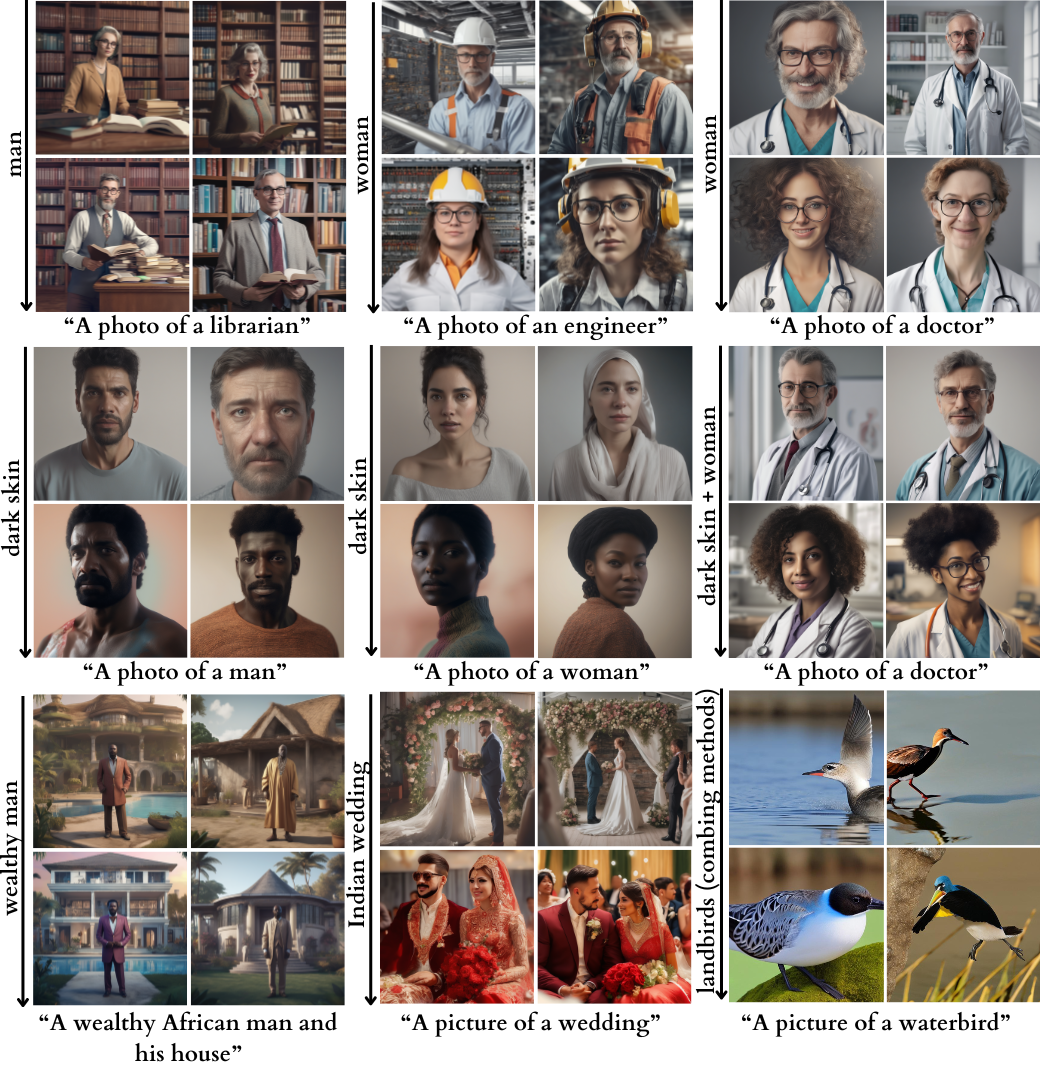
\includegraphics[width=1\linewidth]{images/original_2.png}
   \caption{\textbf{Debiasing diverse concepts.} Generations observed upon the application of our approach in several scenarios.  }
   \label{fig:debiasing_results}
\end{figure}

%The analysis of biases within generative models reveals pervasive biases ranging from gender and race to geographic representation. Notably, Leonardo N. and Dina B. identified concerning patterns in Stable Diffusion v1.5 where low-paying jobs are disproportionately represented by women and darker-skinned individuals. While much research focuses on social and racial biases, Basu et al. conducted a user study validating geographical biases in models like DALLE 2 and Stable Diffusion. Cultural biases were also found, such as in homoglyphs in text-to-image synthesis, where specific characters lead to cultural biases in generated images. Efforts to understand and mitigate biases in vision-language models involve automated gender estimation, face and skin tone detection, and evaluation of geographical representativeness using CLIP-based similarity and k-nearest neighbor models. Debiasing efforts include interventions in prompts, altering prompt embeddings, and leveraging external attribute datasets. Chuang et al.'s method shows promise in improving diversity but operates under assumptions that may not universally hold, while Zhang et al.'s ITI-Gen requires specific attribute datasets and struggles with certain debiasing tasks.

From gender to race, to poor geographic representation, biases can be found everywhere in generative models. Leonardo N. and Dina B. \cite{bloomberg} have found a concerning pattern in Stable Diffusion v1.5 where low-paying jobs are dominated by women and darker-skinned individuals. While most of the work focuses on social and racial biases \cite{bolukbasi2016man, xu2018fairgan}, Basu \textit{et al.} \cite{basu2023inspecting} conduct a user study validating geographical biases in models like DALLE \cite{ramesh2021zeroshot} and Stable Diffusion \cite{rombach2022highresolution}, finding underrepresented 25 out of 27 countries. Cultural biases are also found when using homoglyphs in text-to-image synthesis \cite{mikolov2013exploiting}. Efforts to understand biases in vision-language models lead to the development of automated tools \cite{cho2023dalleval, luccioni2023stable}, the use of gender estimation \cite{li2023blip2}, face and skin tone detection \cite{Bulat_2017, feng2022racially}, and the evaluation of geographical representativeness using CLIP-based similarity and k-nearest neighbor models \cite{basu2023inspecting}. Mitigation efforts include prompt interventions \cite{bansal2022texttoimage}, the development of more inclusive datasets featuring images reflecting diverse geographic and socioeconomic contexts \cite{NEURIPS2022_5474d9d4, ramaswamy2023geode}, and alterations in prompt embedding strategies \cite{chuang2023debiasing, zhang2023itigen}. Chuang \textit{et al.} \cite{chuang2023debiasing} propose a method to mitigate bias by maximizing the similarity between biased and non-biased prompts. They construct a projection matrix to eliminate biased directions from text embeddings before inputting them into the model. Using a similar approach, but employing tokens of available image datasets, ITI-Gen \cite{zhang2023itigen} learns a set of prompt embeddings to append to the initial prompt.

%However, it operates under the assumption the closer the similarity between two text prompts and their embeddings, the more equally represented they should appear on the generated images, which is not a universal truth, being considered a limitation. 


%\textbf{Understanding Vision Language Models.} In an attempt to understand biases in an automated way, Cho \textit{et al.} \cite{cho2023dalleval} use BLIP-2 \cite{li2023blip2} for gender estimation, and FAN \cite{Bulat_2017} and TRUST \cite{feng2022racially} for face and skin tone detection. For automatic evaluation of geographical representativeness, Basu \textit{et al.} \cite{basu2023inspecting} propose CLIP-based similarity between the country specific prompt and the generated image, and k-nearest neighbor model assessing the similarity between a test image and previously annotated images. Luccioni, A. S. \textit{et al.} \cite{luccioni2023stable} introduce three tools to guide in-depth model analysis across biases in professions, a Diffusion Bias Explorer, an Average Face Comparison Tool and two nearest-neighbor lookup tools.

%\textbf{Debiasing Vision Language Models}.  Certain efforts have been directed towards creating more inclusive datasets where images representing geographic and socioeconomic diversity are gathered \cite{NEURIPS2022_5474d9d4, ramaswamy2023geode}. Bansal \textit{et al.} \cite{bansal2022texttoimage} inject ethical interventions into the prompt, such as ”if all individuals can be a [profession] irrespective of their gender”, as a method for combating bias. The state-of-the-art advancements in bias mitigation without requiring additional training or hard prompting, focus on the alteration of prompt embeddings to condition the generations. In these lines, Chuang \textit{et al.} \cite{chuang2023debiasing} maximize the similarity between biased and nonbiased prompts to construct a projection matrix that projects out those biased directions, applied to the text embeddings before feeding them into the model. Their method improves diversity both in their experiments with gender and race, but also generating waterbirds in nonwater backgrounds. However, it operates under the assumption the closer the similarity between two text prompts and their embeddings, the more equally represented they should appear on the generated images, which is not a universal truth, being considered a limitation. In addition to novel work, Zhang \textit{et al.} present ITI-Gen \cite{zhang2023itigen}, leveraging external attribute datasets to learn inclusive tokens that can be combined with the prompt’s embeddings. While the method showcases promising results, it requires a solid dataset of the specific debiasing attribute, failing to handle our experiments debiasing skin tone for the prompt ”A wealthy African man and his house”, proposed by \cite{sunandopaper}, or the Waterbirds benchmark. 

We first present a tool to enhance developers’ visibility, given that we believe understanding the relationship between concepts, and the reason for certain attributes appearing in generations, is key to mitigating them. Secondly, we propose a straightforward novel approach for bias mitigation, linearly separating the latents, noisy information tensors of two different prompts, learning the transformation for debiasing in the latent space of the diffusion model. 

We apply this transformation, named \textit{latent direction}, at a specific weight, linearly combining it with the initial Gaussian noise. The results in a series of diverse experiments prove it successfully works to debias, without the need for prompt alteration. Our approach remains simple, while effective and adaptable to varied scenarios. It allows the synergy of different latent directions, and it is flexible to be used in combination with an approach modifying the prompt embeddings if desired. Through our experiments, we focus on demonstrating the impact of our method for the maximum debiasing transition. However, fair distributions\footnote{Distribution of the generations selected by the user with ethical, truthful, and responsible considerations in mind.} can be obtained when applying the learned latent direction to only a determined percentage of the generations.
 

\section{A Tool for Bias Understanding}
\label{understanding_sec}
Our tool for bias understanding targets two key points: comprehending the connections between embeddings and generations,
and detecting the social characteristics and objects presented in the image. Theoretically, the closer the relation between attribute and concept in the semantic space, the more prone these attributes are to appear in the generated images. We explain the semantic relationship between attributes and concepts by computing the cosine similarity of their embeddings, and comprehending the innate biases within the employed text and vision encoders. In addition, we reveal the visual components of the generated images, using CLIP \cite{radford2021learning} as a zero-shot classifier for gender and race, and Kosmos-2 \cite{peng2023kosmos2} as a Multimodal Large Language Model (MLLM) for perceiving object descriptions from the visual output seen in the images. With this, we present the frequency of objects and social characteristics in the generations, validate if the embedding associations correspond to the visualized content, and provide an understanding of the results without seeing the images. For instance, Fig.~\ref{fig:tool_bias_understanding} informs us that our generations are debiased, with men in suits in front of their houses. However, it presents the innate biases of CLIP's text and vision encoders in Stable Diffusion 2.1 where despite using the prompt \textit{"A \textbf{wealthy} African man and his house"} the highest embedding similarities belong to attributes such as \textit{poverty-stricken} or \textit{underprivileged}. 

\begin{figure}[t]
  \centering
   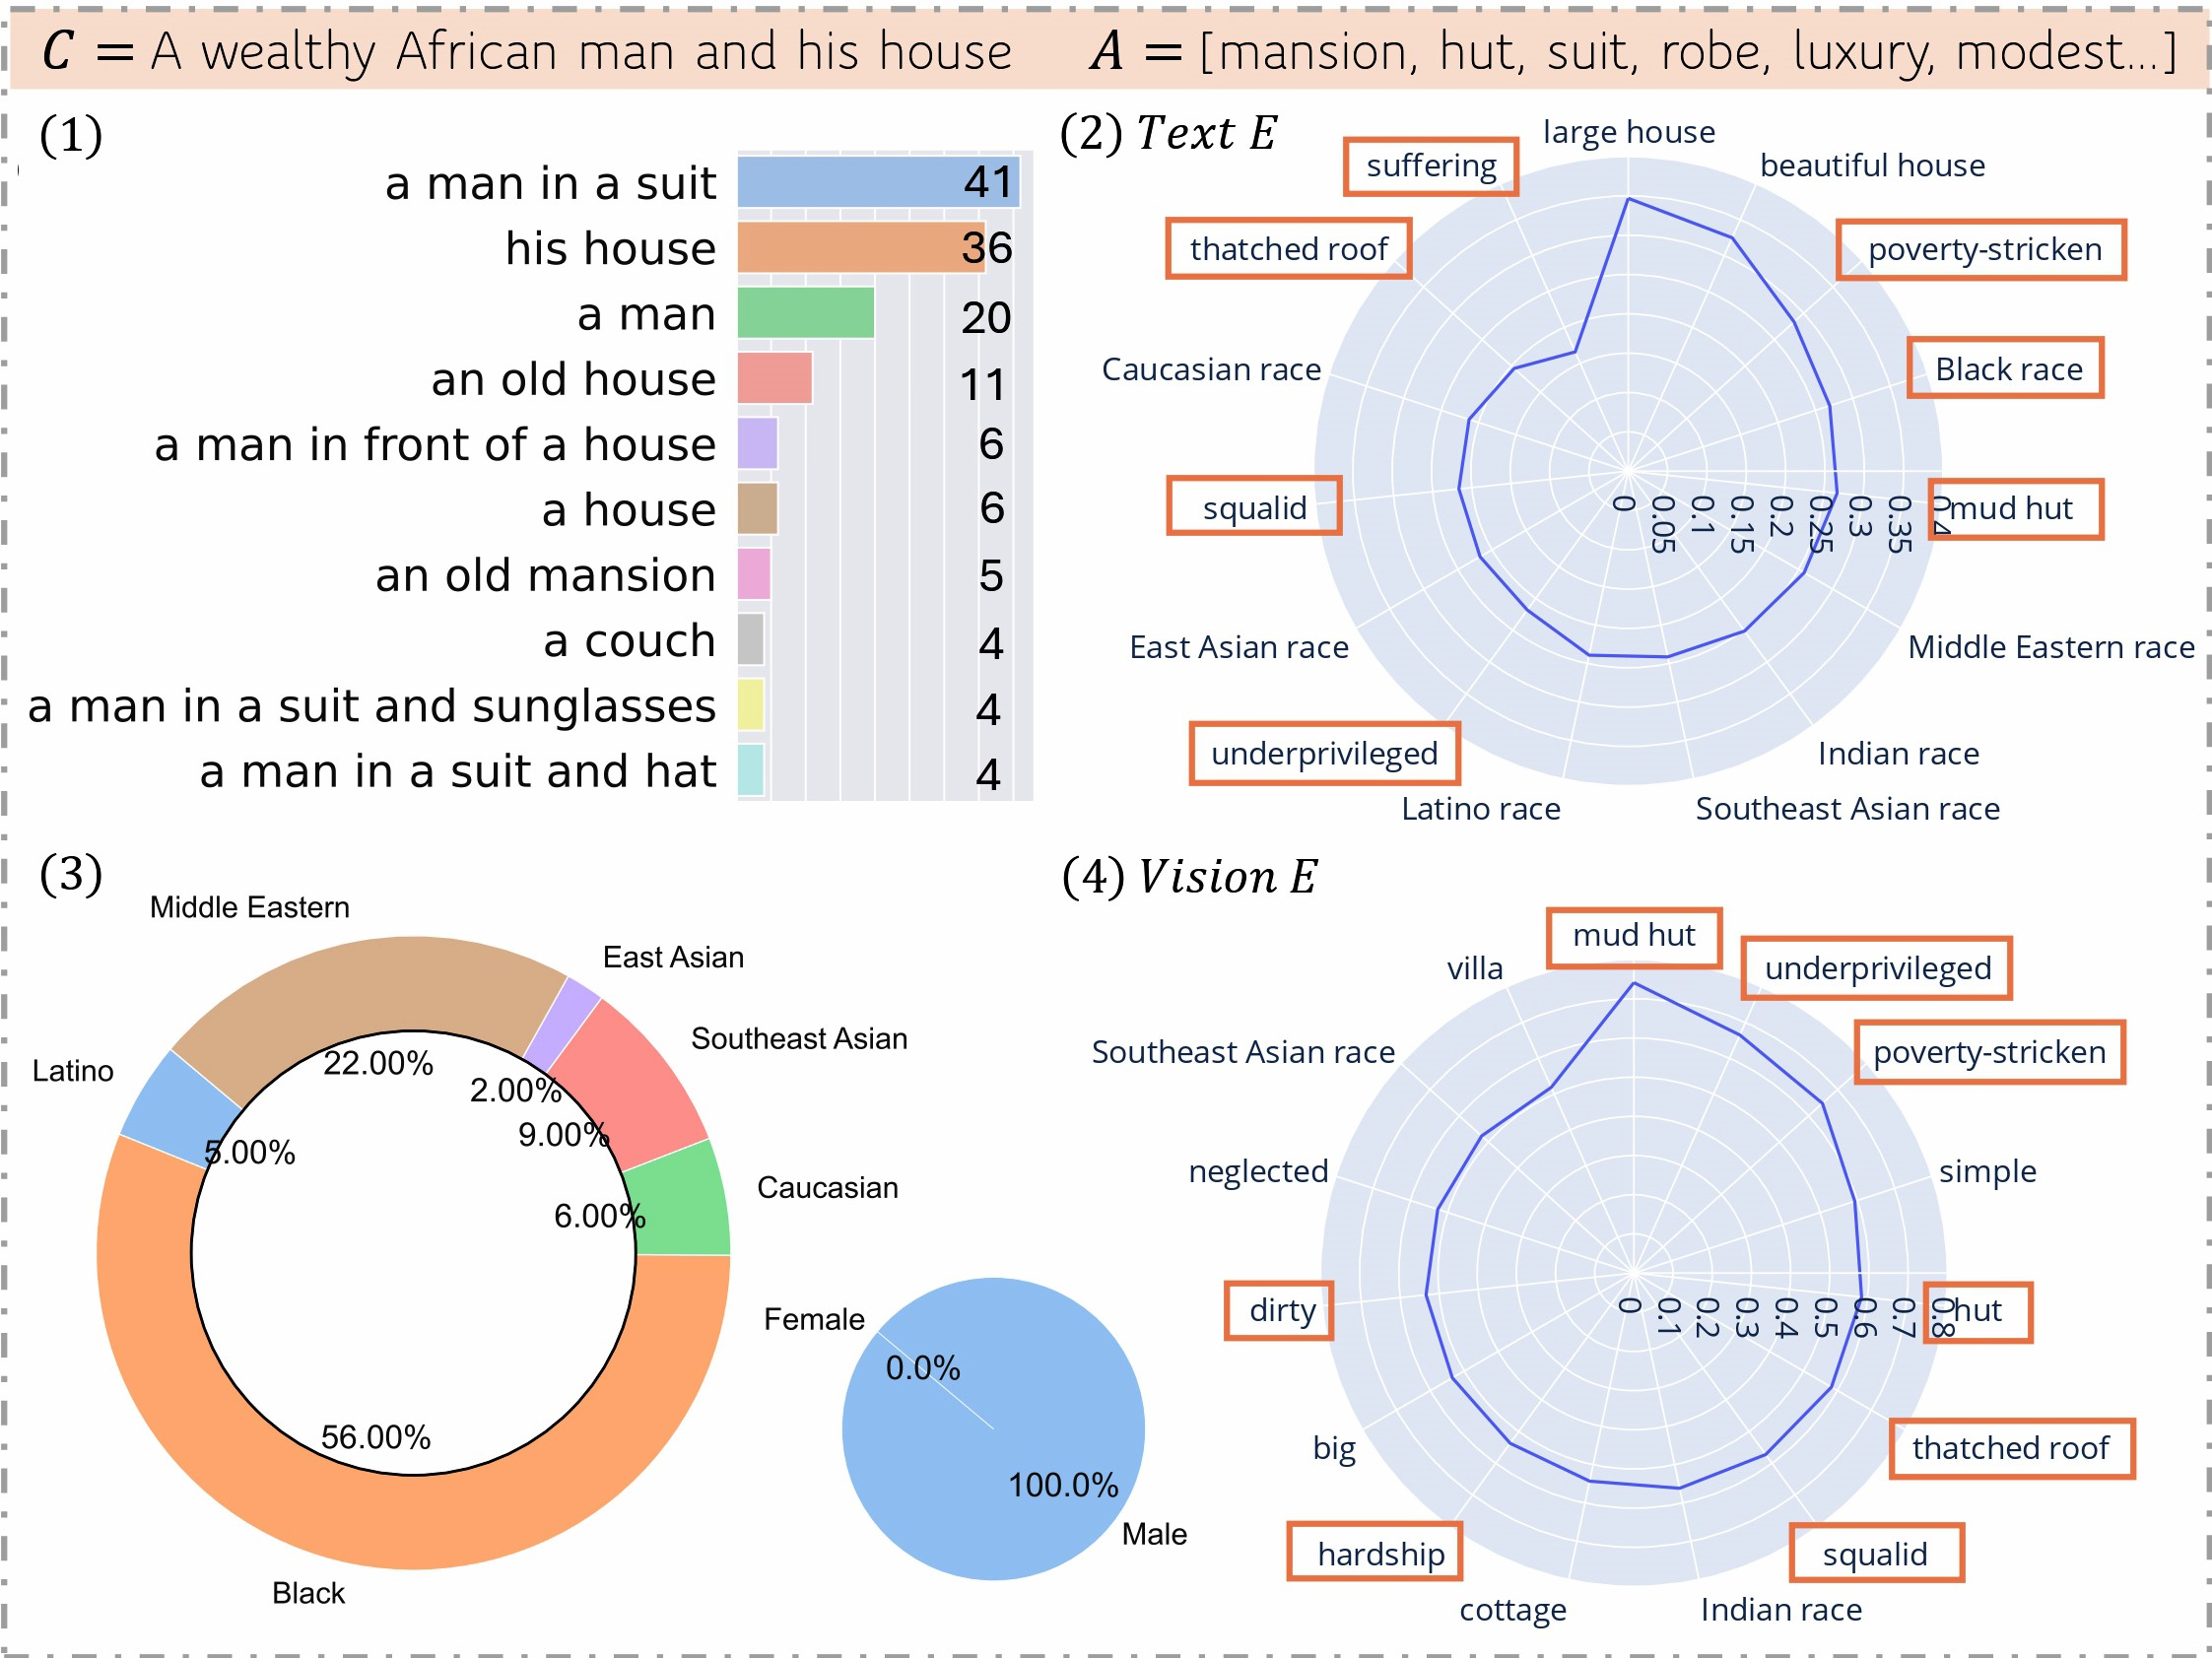
\includegraphics[width=1\linewidth]{images/understanding/understandingToolMama.jpg}
  \caption{\textbf{Example of automated tool output.} Analysis of 100 generations of the concept $C$ across 50 attributes $A$. (1) Frequency count of visual components across the images. (2, 4) Top 15 attributes exhibiting the highest cosine similarity $(C, A)$ across text and vision encoders. (3) Gender and race detections.}
  \label{fig:tool_bias_understanding}
\end{figure}
\section{Our Proposed Method for Bias Mitigation}
\label{mitigation_section}
\begin{figure*}[htb!]
  \centering
   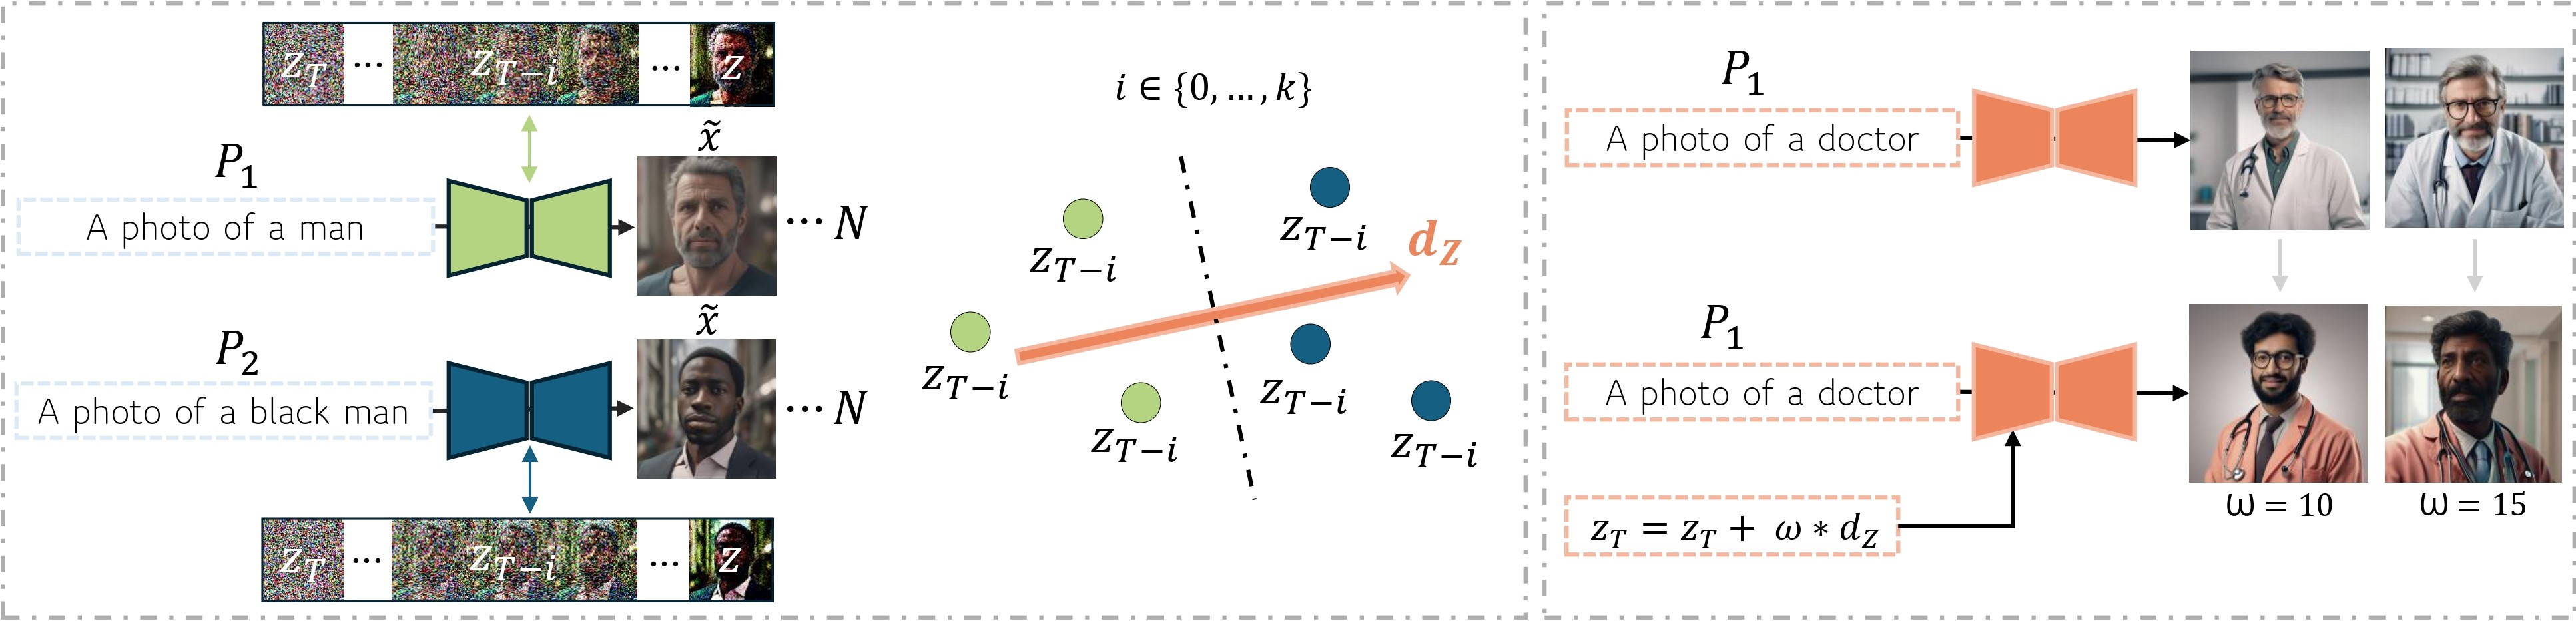
\includegraphics[width=1\linewidth]{images/method_paper_highQ.jpg}
  \caption{\textbf{Summary of our training (left) and inference (right) approach.} We use $P_{1}$ and $P_{2}$ to generate $N$ images $\Tilde{x}$. With their latents, chosen at step $i$, we train a $SVM$ to learn $d_{Z}$. We debias the neutral prompt $P_{1}$, applying $d_{Z}$ to the random initial latent $z_{T} \sim N(\mu, \sigma^2)$ at a specific $\omega$ weight, shifting the generations towards debiased samples with the attributes learned through the latent direction.}
  \label{fig:our_method_training_inference}
\end{figure*}
% Uncomment for a shorter option:
%Previous research in bias mitigation \cite{zhang2023itigen, chuang2023debiasing} focused on the alteration of prompt embeddings to condition the generations. However, given the image arises from the noise distribution [insert appendix], our approach learns the Gaussian Noise direction to condition the initial noise fed into the diffusion process, leaving the original neutral prompt and its embeddings left as is.
\noindent\textbf{Training: Finding the Latent Direction}
Our approach (Fig.~\ref{fig:our_method_training_inference}) proposes a fundamentally different transformation of the diffusion process's input, learning the latent direction $d_{Z}$, from the Gaussian latents at denoised steps, to condition the initial noisy information tensor fed into the diffusion process $z_{T} \sim \mathcal{N}(0, I)$. Given a pre-trained latent diffusion model (LDM) and a neutral prompt $P_{1}$ (\textit{e.g., "a photo of a man, in color, realistic, 8k"}), we aim to obtain debiased generations in the absence of prompt modifications or embeddings alterations. We propose a 'target' prompt $P_{2}$ (\textit{e.g., "a photo of a black man, in color, realistic, 8k"}) and sample $N$ number of images, for both $P_{1}$ and $P_{2}$, to construct the training dataset. The diffusion process for each of the prompts starts from an initial noisy latent  $z_{T}$, which is denoised over $k$ steps, finally reaching the ultimate latent $z$, fed into the decoder $D$ to generate the synthetic image $\tilde{x}$. 

While generating the $N$ images, we save each image's latents at chosen denoising steps $L = (L_{0}, \cdots, L_{k})$, representing ($z_{T},\cdots,z_{T-i}$ for $i \in \{0, 1, 2, \ldots, k\}$ ), building a dataset of noisy information tensors. Note, $L_{0}$ corresponds to the initial Gaussian latent $z_{T}$, while $L_{k}$ is $z$. Once all chosen latents are saved for both prompts, we select one denoising step $i$ to obtain $d_{Z}$ with those specific latents. For instance, we could decide to train with $L_{10}$, the latents saved for the $N$ images at step 10 ($z_{T-10}$). 

\noindent\textbf{The model.} We use a support vector machine (SVM) \cite{Vapnik2015} to linearly separate the latents across our labeled dataset of $N$ samples for each prompt. The classifier uses a linear kernel and provides the $d_{Z}$, the so-called \textit{latent direction}, we utilize for debiasing. 


\noindent\textbf{Inference: Applying the Latent Direction.}
To obtain debiased generations, the LDM, in our case Stable Diffusion \cite{rombach2022highresolution}, uses for inference only $P_{1}$, the neutral prompt. This prompt is fed into CLIP's text encoder $E$ forming the first input. As the second one, instead of using an initial Gaussian random information tensor for denoising, we transform this latent by applying the learned latent direction $d_{Z}$, following equation \ref{eq:important}. 

\begin{equation}
  z_{T} = z_{T} + \omega \cdot d_{Z}
  \label{eq:important}
\end{equation}

Where $z_{T} \sim N(\mu, \sigma^2)$ and $\omega$ is the weight parameter at which the latent direction is applied. The higher the $\omega$, the higher the strength of the debiasing impact. 


%the other approaches inject the learned tokens or jiggle around these embeddings. 
% There is a tradeoffinvolved in finding the optimal latent to train the classifier. Out of 50 denoising steps

%We refer to this direction as \textit{latent direction} and to learn it, we utilize Stable Diffusion to generate two datasets of 50 samples each, using the neutral and the debiased prompt. The relevant part of these datasets are not the final generated images, but the noise latents involved in their denoising processes. In our case we have used 50 denoising steps, saving these latents every 5th step, obtaining 9 latents [L5, L10, L15 … L45] per image. For training, one of these latent steps is selected and fed as input data for a Support Vector Machine (SVM) classifier with a linear kernel.  The SVM provides two learned latent directions, the biased and debiased ones. As a result, to successfully mitigate biases we use the original neutral prompt, linearly combining the initial Gaussian noise with the weighted latent direction, following: 


\noindent\textbf{The optimal configuration.} Optimal debiasing results are found when selecting the most favorable latent $L = (L_{0}, \cdots, L_{k})$ and weight configuration $\omega$. Thus, we propose two approaches to automatically find it without having to visually explore all possibilities. The first one is to use the \textit{clean-fid} \cite{parmar2022aliased} library to compute the similarity between the distribution of a small subset of generated images with a particular configuration, and the distribution of known debiased images, and the second one is to leverage CLIP \cite{radford2021learning} as a zero-shot classifier, selecting the configuration with a high classification of the desired debiased class. 
%We find the effectivity of our method is conditioned upon the selection of the latent $L = (L_{0}, \cdots, L_{k})$ and weight configuration $\omega$, given each debiasing scenario has its own, and optimal debiasing results are achieved when found.

\section{Experimental Results}
\label{mitigation_results_section}

% \begin{table*}[hbt!]
%   \centering
%     \begin{tabular}{l|cc|ccc|c|c|c}
%     \hline $d_{Z}$ &\multicolumn{2}{|c}{ Dark Skin Tone } & \multicolumn{3}{c}{Female Gender } & \multicolumn{1}{|c}{ Landbird } & \multicolumn{1}{|c}{ Indian } & \multicolumn{1}{|c}{ Wealthy man }\\
%      $P_{1}$ & Man & Woman & Doctor & Firefighter & Cleaner & Waterbird  & Wedding & African man\\ 
%     \hline SD XL & 8\% & 1\% & 0\% & 14\% & 65\% & 25\%  & 0\% & 38\%\\
%     Ours & 92\% & 79\% & 52\% & 22\% & 56\% & 25\% & 33\% & 10\%\\
%     SD 2.1& 6 & 0 & 14 & 27\% & 46 & 25 & 0 & 4\\
%     Debias VL & 88 & 78.7 & 28 & 33 & 47 & 50 & 0 & 51\\
%     Combination & 100 & 100 & 47 & 68 & 23 & 0 & 0 & 51\\
%     \hline
%     \end{tabular}
%     \caption{\textbf{Quantitative results.} Comparison of generations prior and post debiasing using the latent direction $d_{Z}$ learned for dark skin tone transition, }
% \end{table*}

We validate our work using Stable Diffusion XL \cite{rombach2022highresolution}, with $50$ denoising steps, applying different latent directions $d_{Z}$ in a series of experiments to understand its impact. Successful results are obtained in diverse mitigations. We present four different debiasing scenarios following the settings of previous papers \cite{chuang2023debiasing, zhang2023itigen, jain2021imperfect, friedrich2023fair}, addressing social group biases, cultural and geographical biases, and the Waterbird \cite{sagawa2020distributionally} benchmark for evaluating spurious correlations. Fig.~\ref{fig:debiasing_results} summarizes the experimental results obtained.

\noindent\textbf{Quantitative Metrics.} We leverage the Statistical Parity Difference ($SPD$) \cite{dwork2011fairness} to evaluate our debiasing method in the generated image datasets. We use CLIP for attribute prediction and measure the absolute difference in the proportions of desired attributes between the original biased dataset, generated with the plain Stable Diffusion model, and the debiased dataset. A value close to zero indicates minimal debiasing impact, while a value of one signifies successful debiasing with the desired attribute present in all generations. 

%Additionally, we quantify image quality using the FID score \cite{zhang2023itigen} through the \textit{clean-fid} library \cite{parmar2022aliased}. 

\begin{table*}[ht!]
  \centering
    \begin{tabular}{l|cc|ccc|c|c|c}
        \hline
        $d_{Z}$ & \multicolumn{2}{c|}{\textbf{Skin Tone}} & \multicolumn{3}{c|}{\textbf{Gender}} & \textbf{Landbird} & \textbf{Indian} & \textbf{Wealth}\\
        \textit{$P_{1}$} & \textit{Man} & \textit{Woman} & \textit{Doctor} & \textit{Firefighter} & \textit{Cleaner} & \textit{Waterbird}  & \textit{Wedding} & \textit{African man}\\
        \hline 
         (SD XL, ours) & 0.87 & 0.78 & \textbf{0.52} & \textbf{0.08} & 0.09 & - & 0.33 & 0.28\\
         % 0.08 for watrbirds using sd21
        (SD 2.1, PD \cite{chuang2023debiasing})  & 0.91 & 0.90 & 0.14 & 0.06 & 0.01 & 0.29 & 0.79& 0.47\\
        (SD 2.1, ours + PD \cite{chuang2023debiasing}) & \textbf{0.94} & \textbf{1.00} & 0.29 & 0.04 & \textbf{0.22} & \textbf{0.68} & \textbf{1.00} & \textbf{0.96}\\
        \hline
    \end{tabular}
    \caption{\textbf{Quantitative results across 100 generations.} $SPD$ in the presence\protect\footnotemark of the desired attributes: dark skin tone, female gender for the case of \textit{doctor, firefighter} and male gender for \textit{cleaner}, land environments for waterbirds, Indian wedding attributes and wealthier looking houses avoiding thatched roofs and mud huts. We learn the latent directions with SD 2.1 for the results seen in the last row.}
    \label{table_quantitative_results}
\end{table*}

\noindent\textbf{Gender debiasing in professions.} We learn $d_{Z}$ by defining $N=50$, $P_{1}=$\textit{"a photo of a man, in color, realistic, 8k"} and $P_{2}=$\textit{"a photo of a woman, in color, realistic, 8k"}, selecting $L_{25}$ and $\omega=10$. We apply the \textit{woman} latent direction to the neutral prompts \textit{“a photo of a [profession], in color, realistic, 8k”} and observe a positive shift from 0\% to 52\%, in 100 generations for the case of "doctor". Other professions known to be extremely biased, such as firefighter, engineer, or librarian have shown a slightly improved impact, with shifts of 8\%, 3\%, and 2\%, respectively. We believe major debiasing can be achieved with these professions upon finding the optimal $d_{Z}$.

%towards women subjects in the evaluated professions, with extremely good results for the concept of \textit{doctor}. 


\noindent\textbf{Skin tone debiasing.} We explore the transition of skin tones in generated images. For it, we create four training datasets, where $N=50$, with $P_{1}=$\textit{”a photo of a [man/woman], in color, realistic, 8k”} and $P_{2}=$\textit{”a photo of a black [man/woman], in color, realistic, 8k.”}. With the proposed automated method for configuration selection we settle on training with the latents at step 10 ($L_{10}$), at a weight $\omega=15$. The results shift 100 generations using the neutral prompt $P_{1}=$\textit{”a photo of a man, in color, realistic, 8k”} to contain a 95\% of black men images from the original 8\%. Similarly, with $P_{1}=$\textit{”a photo of a woman, in color, realistic, 8k”} and the application of the dark-skin $d_{Z}$ at $L_{25}$, $\omega=14$ yields a 79\% of black women from an initial 1\%.

\noindent\textbf{Waterbird debiasing.} In this experiment we evaluate the impact of the combination of methods, manipulating both the prompt’s embeddings \cite{chuang2023debiasing} and the initial Gaussian noise, using Stable Diffusion 2.1. We aim to generate waterbirds in land environments with the prompt $P_{1} =$ \textit{"A picture of a waterbird"}. We replicate their setup and apply our learned latent direction ($P_{1} =$ \textit{"A picture of a waterbird"}, $P_{2} =$ \textit{"A picture of a landbird"}, $\omega=10$, $L_{10}$). The results across 100 generations yield exceptional results with 78\% of generations displaying waterbirds in terrestrial habitats, 2\% in aquatic landscapes, and 20\% showing bird portraits.

%are classified using CLIP with 3 different pairs of prompts: \textit{[”A bird floating in water”, ”A bird standing out of the water”], [”A bird walking on water”, ”A bird walking on land.”], and [”A picture of a waterbird.”, ”A picture of a landbird.”]}. The scores are compared to their method \cite{chuang2023debiasing} following the same setup used in their experiments. Given both approaches are fundamentally different, we combine the methods,  The integration of both methodologies yields superior performance, as evidenced in Figure \ref{comparison_waterbirds}[TO FIX]. 

% \begin{figure}[t]
%   \centering
%    \includegraphics[width=1\linewidth]{images/waterbirds_boxplot.png}
%    \caption{\textbf{Boxplot comparison between the original generations, the individual approaches, and the combination of both.} The figure reflects the performance observed using the three proposed classification prompts. Combination of both approaches enhances their approach to reach the best performance.}
%    \label{comparison_waterbirds}
% \end{figure}

\noindent\textbf{Geographical representativeness.} It is hard to obtain balanced geographical representations of \textit{”a picture of a wedding, in color, realistic, 8k}”, given this neutral prompt is normally biased towards representations of Western weddings. In an attempt to shift the distribution towards Indian weddings, we define $P_{1}=$\textit{”a picture of a wedding, in color, realistic, 8k”} and $P_{2}=$\textit{”a picture of a wedding in India, in color, realistic, 8k”}, learning $d_{Z}$ using $L_{30}$ and applying it with $\omega=35$ we see an increment of 33\% in CLIP's classification. Inspired by Bianchi \textit{et al.} \cite{sunandopaper} we debias 38\% of the thatched roofs observed when using $P_{1}$=\textit{"A wealthy African man and his house"}, utilizing $P_{2}$=\textit{"A wealthy man and his house"} and applying the learned \textit{wealthy man} direction $d_{Z}$ at $L_{10}$ and $\omega=15$.

\noindent\textbf{Comparison with PD.} In Tab.~\ref{table_quantitative_results}, we present the quantitative results of our study. The comparison with the Prompt Debiasing (PD) method~\cite{chuang2023debiasing} is challenging, due to the utilization of distinct models and the diverse biases in them, e.g., for $P_{1}=$\textit{"A wealthy African man and his house"} SD XL presents generations of mansions with thatched roofs, whereas SD 2.1 shows mud huts. We choose to use SD XL given the enhanced quality of the model facilitates the learning of $d_{Z}$ and minimizes the inconveniences of elaborated hard prompting to obtain quality images with SD 2.1. The outcomes evaluated through our experiments demonstrate the potential of latent directions to obtain competitive debiased generations despite maintaining neutral embeddings. 

  % e.g. for $P_{1}=$"A wealthy African man and his house" SD XL presents generations of mansions with thatched roofs, whereas SD 2.1 shows mud huts. Comparison to PD is hard given the models desparities.
\subsection{Relevant Insights and Learnings}
The integration of prompt debiasing and latent directions surpasses the efficacy of the former used individually (Tab.~\ref{table_quantitative_results}). Regarding our approach, the results in Fig.~\ref{fig:gallery_black_woman} confirm the choice of weight $\omega$ has a higher impact on the debiasing than the choice of training latent $L$. Moreover, higher latent directions require lower weights to achieve the debiased results, given more structured noise is found at the higher debiasing steps. However, as we move in $d_{Z}$ there is a limit to how far we go with $\omega$, given an extremely high weight leads to distorted generations, out of the distribution. Lastly, it is possible to linearly combine latent directions following $z_{T} = z_{T} + \sum_{i=1}^{\infty} \omega_{i} \cdot d_{Zi}$. For instance, by applying the \textit{woman} [$L_{25}$ $\omega10$] and \textit{dark-skin} [$L_{10}$ $\omega10$] latent directions to the Gaussian noise of the neutral prompt $P_{1}=$\textit{“a photo of a doctor, in
color, realistic, 8k”} we achieve generations of dark-skinned female doctors (Fig.~\ref{fig:debiasing_results}).

\begin{figure}[t]
  \centering
   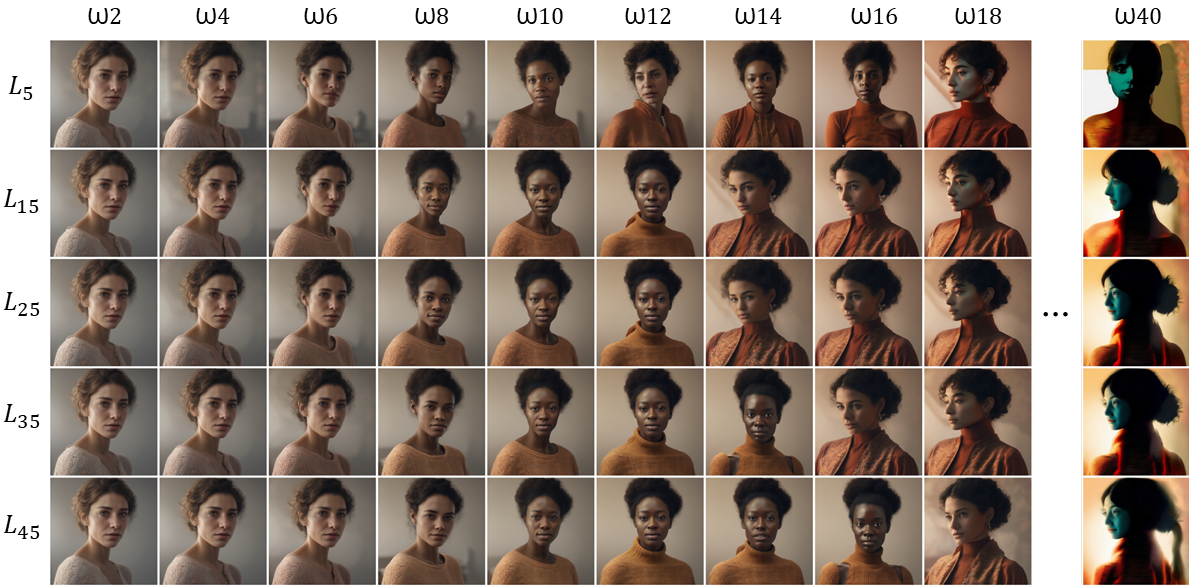
\includegraphics[width=1\linewidth]{images/weight_latent_transition.png}

   \caption{\textbf{Comparison of results with $d_{Z}$ trained at different latents $L$ and applied at different weights $\omega$.} Generations of the same woman in its transition to dark skin.}
   \label{fig:gallery_black_woman}
\end{figure}

\footnotetext{Presence of classes through CLIP's classification: ["A picture of a black [man/woman]", "A picture of a white [man/woman]"], ["A picture of a woman", "A picture of a man"], ["A picture of a Western wedding", "A picture of an Indian wedding"]. A user study is used to evaluate the complex generations (\textit{Wedding}, \textit{African man}) given classification with defined classes in these cases does not match reality.}


%We leverage the discrepancy metric used by \cite{chuang2023debiasing},the L2 norm between empirical and uniform distributions. 

% We use two metrics to quantify distribution diversity and image quality. (1) Distribution Discrepancy (DKL). 



\section{Conclusion}
After proposing a tool for uncovering and quantifying the present bias in text-to-image models, a novel method is proposed for mitigation. By learning and applying latent directions $d_{Z}$ we demonstrate it is possible to alter the diverse complex biased relations, such as those in cultural events, while maintaining unaltered neutral prompt embeddings. \textbf{Future work} encourages the exploration of more advanced classifiers to find the optimal $d_{Z}$.

%However, our methodology presents the potential impact the initial random Gaussian noise has in these modifications.

% design of more complex models to learn the latent direction

% Moreover, it has demonstrated remarkable adaptability to the diverse challenges of the evaluation directions, being adaptable from gender and race to cultural events and object debiasing.


{
    \small
    \bibliographystyle{ieeenat_fullname}
    \bibliography{main}
}

% WARNING: do not forget to delete the supplementary pages from your submission 
%\input{sec/X_suppl}

\end{document}
